% THIS DOCUMENT IS FOLLOWS THE VOLERE TEMPLATE BY Suzanne Robertson and James Robertson
% ONLY THE SECTION HEADINGS ARE PROVIDED
%
% Initial draft from https://github.com/Dieblich/volere
%
% Risks are removed because they are covered by the Hazard Analysis
\documentclass[12pt]{article}

\usepackage{booktabs}
\usepackage{tabularx}
\usepackage{graphicx}
\usepackage{hyperref}
\usepackage{booktabs}
\usepackage{geometry}
\usepackage{caption}
\usepackage{longtable}
\usepackage{multirow}
\usepackage{graphicx}
\hypersetup{
    bookmarks=true,         % show bookmarks bar?
      colorlinks=true,      % false: boxed links; true: colored links
    linkcolor=red,          % color of internal links (change box color with linkbordercolor)
    citecolor=green,        % color of links to bibliography
    filecolor=magenta,      % color of file links
    urlcolor=cyan           % color of external links
}

\newcommand{\lips}{\textit{Insert your content here.}}

%% Comments

\usepackage{color}

\newif\ifcomments\commentstrue %displays comments
%\newif\ifcomments\commentsfalse %so that comments do not display

\ifcomments
\newcommand{\authornote}[3]{\textcolor{#1}{[#3 ---#2]}}
\newcommand{\todo}[1]{\textcolor{red}{[TODO: #1]}}
\else
\newcommand{\authornote}[3]{}
\newcommand{\todo}[1]{}
\fi

\newcommand{\wss}[1]{\authornote{blue}{SS}{#1}} 
\newcommand{\plt}[1]{\authornote{magenta}{TPLT}{#1}} %For explanation of the template
\newcommand{\an}[1]{\authornote{cyan}{Author}{#1}}

%% Common Parts

\newcommand{\progname}{McMaster Engineering Society Custom Financial
Expense Reporting Platform} % PUT YOUR PROGRAM NAME HERE
\newcommand{\authname}{Team \#12, Reimbursement Rangers
\\ Adam Podolak
\\ Evan Sturmey
\\ Christian Petricca
\\ Austin Bennett
\\ Jacob Kish} % AUTHOR NAMES                  

\usepackage{hyperref}
    \hypersetup{colorlinks=true, linkcolor=blue, citecolor=blue, filecolor=blue,
                urlcolor=blue, unicode=false}
    \urlstyle{same}
                                


\begin{document}

\title{Software Requirements Specification for \progname: (Volere)} 
\author{\authname}
\date{\today}
	
\maketitle

~\newpage

\pagenumbering{roman}

\tableofcontents

~\newpage

\section*{Revision History}

\begin{table}[htp]
\centering
\caption{Revision History}
\label{TblRevisionHistory}
\begin{tabularx}{\textwidth}{l l l X}
\toprule
\textbf{Date} & \textbf{Developer(s)} & \textbf{Commit} & \textbf{Change}\\

\midrule
10/11/24 & 
All Team Members & 
\href{https://github.com/ausbennett/mes-finance-platform/pull/21}{Pull Request 21} & 
All sections, including reflections\\

\midrule
1/6/25 & 
  Adam Podolak, Austin Bennett & 
\href{https://github.com/ausbennett/mes-finance-platform/commit/645f5a5ecfee7cc2adbb784888d733d815d3080f}{645f5a5}, \href{https://github.com/ausbennett/mes-finance-platform/commit/55fbc0d26a10b56f90c50919de7a8c9ca920ec11}{55fbc0d}  & Making the constraints list bulleted, expanded on off-the-shelf choices. \\

\bottomrule
\end{tabularx}
\end{table}

~\\

~\newpage
\section{Purpose of the Project}
\subsection{User Business}
The project aims to streamline the process of handling reimbursement requests for the McMaster Engineering Society, facilitating proper budget tracking, improved efficiency and user experience, as well as reducing human error.

\subsection{Goals of the Project}
Goals include:
\begin{itemize}
    \item User-friendly reimbursement submission interface.
    \item Tracking of reimbursement requests.
    \item Tiered access to the reimbursement platform for different users.
    \item Invoice generation.
\end{itemize}

\section{Stakeholders}
\subsection{Client}
This software is designed for the McMaster Engineering Society and its personnel, and by extension for McMaster University.

\subsection{Customer}
MES clubs/team members that are required to submit reimbursement requests for their projects and club work.

\subsection{Other Stakeholders}
University administration, future developers of the finance platform, and outside auditors.

\subsection{Hands-On Users of the Project}
Day to day, the software will be used by students submitting reimbursement requests for themselves or on their teams' behalf, as well as MES finance personnel who are to review requests and handle them accordingly.

\subsection{Personas}
\begin{itemize}
    \item \textbf{Club Treasurers}: Needs to be able to submit reimbursement requests easily and frequently, as well as track the status of requests.
    \item \textbf{Finance personnel}: Needs to be able to effectively manage all incoming reimbursement requests from different clubs/users.
    \item \textbf{Club Member/General Students}: Infrequent reimbursement request submission; user-friendliness is required.
    \item \textbf{Auditor}: Needs ready access to necessary financial documentation submitted to and generated by the finance platform.
\end{itemize}

\subsection{Priorities Assigned to Users}
Highest to Lowest:
\begin{enumerate}
    \item MES Finance personnel
    \item Club Treasurers
    \item Club Members/General Students
    \item Auditors
\end{enumerate}

\subsection{User Participation}
User testing will be conducted with Club Treasurers/Club Members as well as the MES Finance personnel to ensure requirements are met.

\subsection{Maintenance Users and Service Technicians}
MES personnel will maintain the system after its deployment.


\section{Mandated Constraints}
\subsection{Solution Constraints}
\begin{itemize}
    \item The finance platform will adhere to the data privacy regulations of McMaster University.
    \item The finance platform will integrate with existing McMaster IT infrastructure.
    \item The finance platform will only be available to McMaster affiliated individuals, including students, team/club members, treasurers, MES finance personnel, McMaster Administration, and outside auditors.
\end{itemize}

\subsection{Implementation Environment of the Current System}
\begin{itemize}
    \item The current system operates using a combination of Google Forms submissions and Google Sheets for tracking. 
    \item MongoDB is used for database management, and Digital Ocean is used for cloud management.
\end{itemize}

\subsection{Partner or Collaborative Applications}
\begin{itemize}
    \item While the finance platform will involve a technology stack, it will be standalone in its operations.
    \item It will integrate with existing MES IT infrastructure but will wholly replace the existing reimbursement platform.
\end{itemize}
 

\subsection{Off-the-Shelf Software}
The team has decided that we will not be integrating any off-the-shelf solutions at this time.

\begin{itemize}
    \item Some existing off-the-shelf solutions include Intuit QuickBooks and Xero.
    \item QuickBooks could be used for ledger tracking and invoice generation, while Xero can also streamline the invoice process.
    \item The team has decided against integrating off-the-shelf solutions as they would introduce extra risks that do not offset the benefit they would bring. 
\end{itemize}
 
\subsection{Anticipated Workplace Environment}
\begin{itemize}
    \item The finance platform will primarily be accessed online via a website. Mobile access will also be possible. 
    \item Although access will be restricted to McMaster affiliated individuals, the platform will be accessible from anywhere.
\end{itemize}
 

\subsection{Schedule Constraints}
\begin{itemize}
    \item The finance platform must be completed by the end of the Winter 2025 term; however, completing it sooner is ideal to address existing MES finance concerns.
\end{itemize}


\subsection{Budget Constraints}
\begin{itemize}
    \item The project at this stage is not projected to require additional funds.
\end{itemize}

\subsection{Enterprise Constraints}
\begin{itemize}
    \item As previously mentioned, the finance platform must adhere to McMaster University’s data privacy regulations and cybersecurity standards.
\end{itemize}

\section{Naming Conventions and Terminology}
\subsection{Glossary of All Terms, Including Acronyms, Used by Stakeholders Involved in the Project}
\begin{table}[h]
    \centering
    \begin{tabular}{|>{\raggedright}p{3cm}|>{\raggedright\arraybackslash}p{10cm}|}
        \hline
        \textbf{Term} & \textbf{Definition} \\
        \hline
        MES & McMaster Engineering Society \\
        \hline
        IT & Information Technology \\
        \hline
        UAT & User Acceptance Testing \\
        \hline
        API & Application Programming Interface \\
        \hline
        UI & User Interface \\
        \hline
        CTA & Call-to-Action – an element of a web-page that elicits an action from the user \\
        \hline
        FAQ & Frequently asked questions \\
        \hline
    \end{tabular}
    \caption{Glossary of Terms and Acronyms}
    \label{tab:glossary}
\end{table}


\section{Relevant Facts And Assumptions}
\subsection{Relevant Facts}
The current MES reimbursement process relying on Google Forms and Google Sheets has proven cumbersome, and as a result, students are not inclined to make timely reimbursement requests, introducing avoidable problems to the finance team.
The MES does not receive its due fees from McMaster University unless they pass their audits, making the process of submitting reimbursement requests integral to the MES staying operational and receiving its due funding.
Outside of efficiency and availability, the existing platform also does not include enough tracking/updates along the journey of a given request, making some information susceptible to being lost.

\subsection{Business Rules}
\begin{itemize}
    \item All reimbursement requests must include a receipt or invoice as proof of purchase.
    \item The MES Finance team has the authority to modify the reimbursement process as needed to handle extraneous circumstances.
    \item The platform’s functionality is subject to change in the future as per the needs of the MES.
\end{itemize}

\subsection{Assumptions}
\begin{itemize}
    \item Unless otherwise stated, the MES finance team will be able to review requests in a fixed, predetermined timeline.
    \item Reimbursement requests can only be made with all requisite information and documentation.
    \item Reimbursement requests will only be made from MES Clubs/Teams to the MES.
    \item Internet access will be required to use the finance platform.
    \item All data submitted to the platform will be securely stored.
    \item All users accessing the platform will have to verify themselves to gain aceess.

    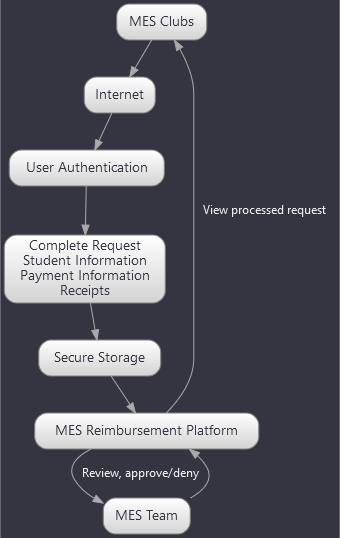
\includegraphics[width=0.8\textwidth]{imgs/assumptions.png}
\end{itemize}


\section{The Scope of the Work}

\subsection{The Current Situation}
The McMaster Engineering Society (MES) currently manages financial reporting, reimbursements, and expense tracking through a disjointed system involving Google Forms, PDFs, and spreadsheets. This fragmented approach leads to inefficiencies, delays in reimbursements, errors, and increased administrative burden. MES requires a streamlined platform to centralize these processes, ensuring compliance with audit standards and reducing the time spent on financial management tasks.

\subsection{The Context of the Work}
The MES supports around 60 student groups and numerous individuals, organizing various academic, professional, and recreational activities. Effective financial management is essential for ensuring that these student groups receive timely funding and reimbursements. Without an efficient system, MES risks delayed payments, financial inaccuracies, and non-compliance with audit requirements. Developing a centralized platform is critical for MES to continue supporting student initiatives and ensuring smooth financial operations.

\begin{figure}[h!]
    \centering
    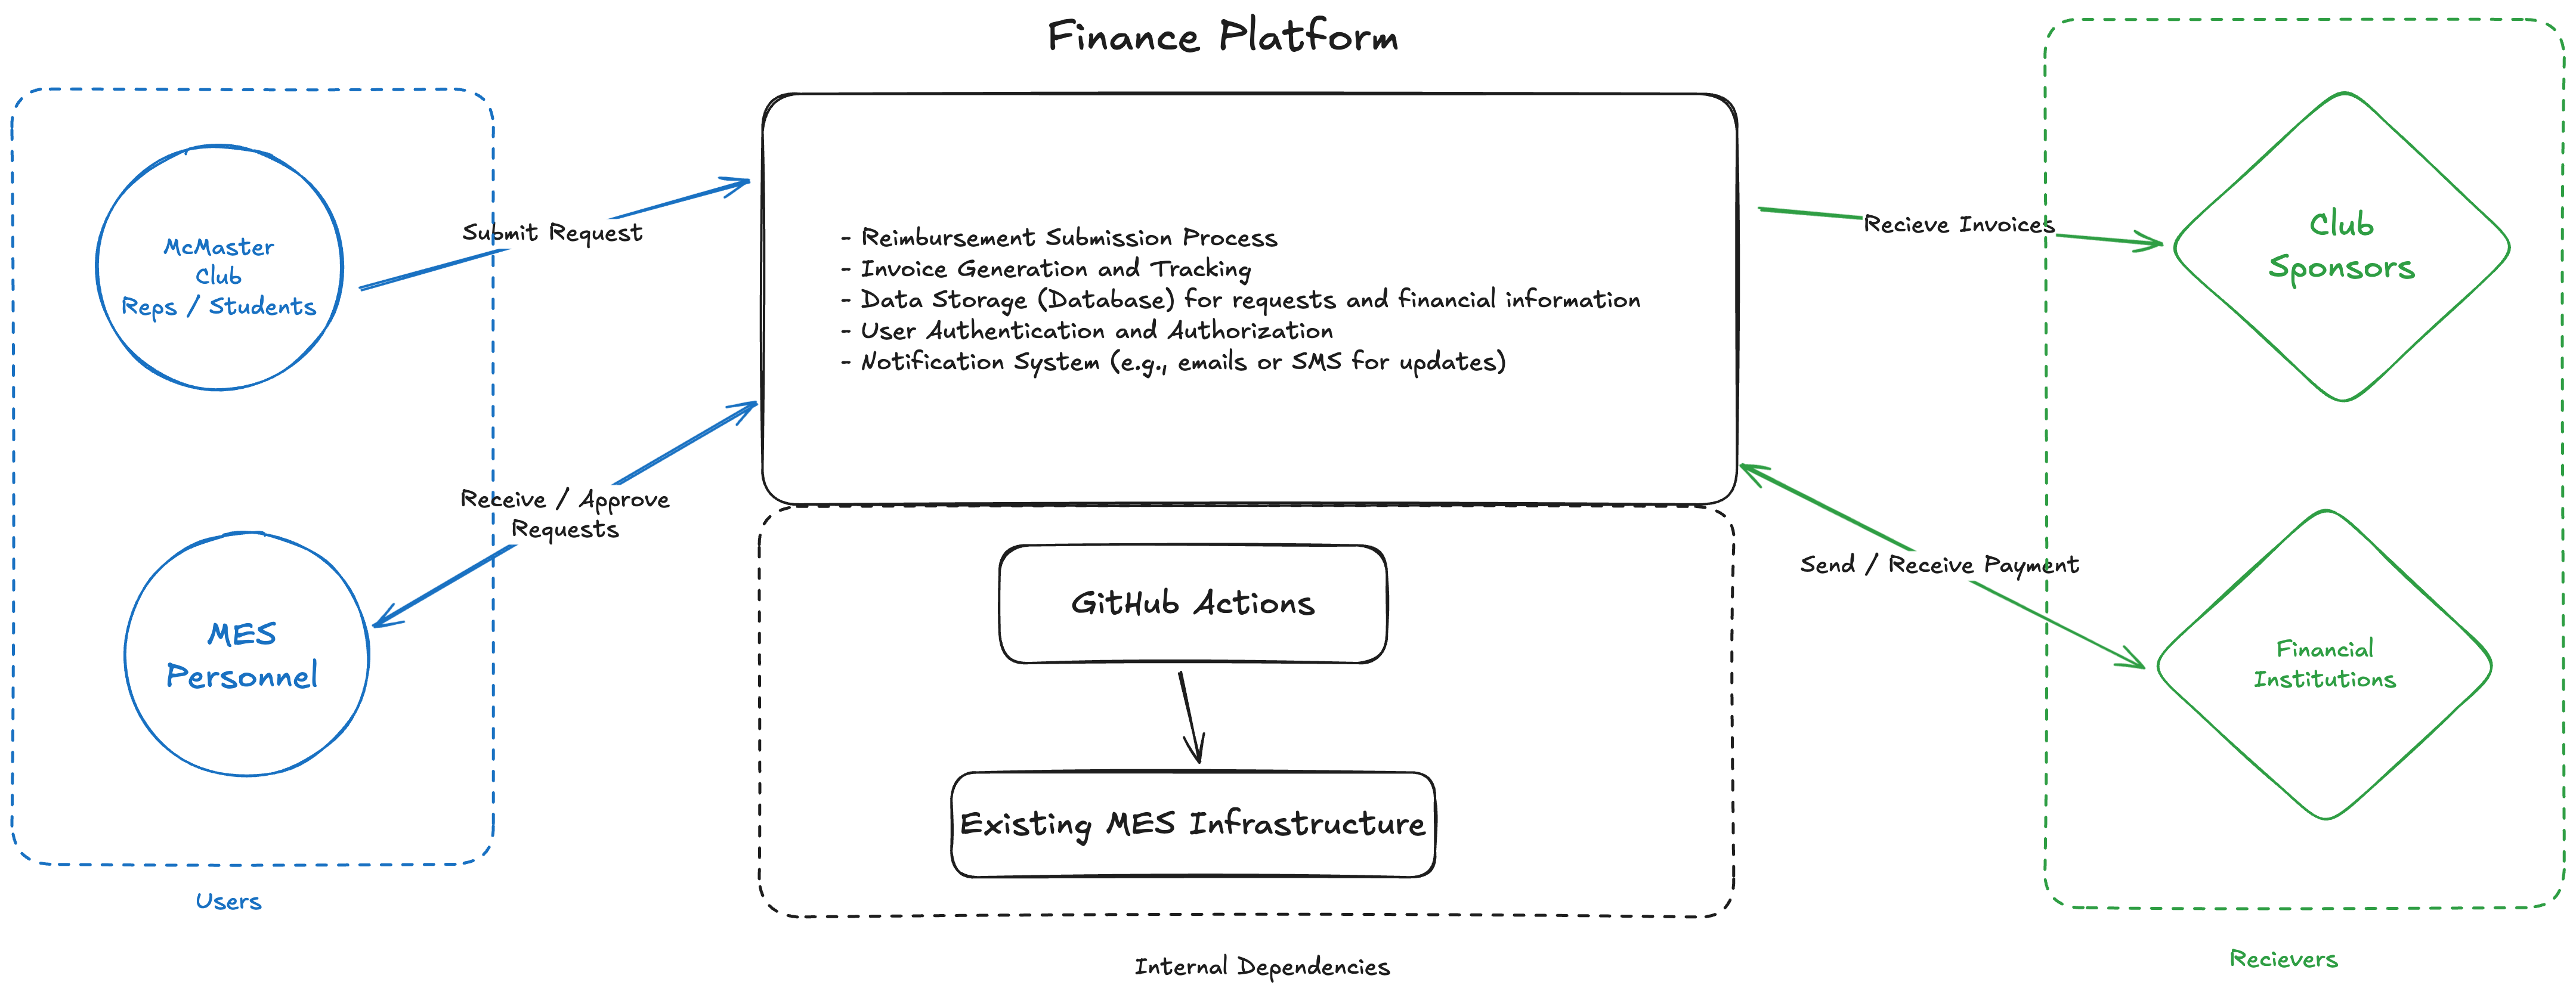
\includegraphics[width=0.8\textwidth]{./imgs/context-diagram.png}
    \caption{Context Diagram}
\end{figure}



\subsection{Work Partitioning}
The project will be divided into the following key tasks:
\begin{itemize}
    \item \textbf{Research and Requirements Gathering:} Analyze current MES workflows and identify the specific financial management needs of the organization.
    \item \textbf{Design and Architecture:} Create the architecture for a centralized financial platform, focusing on scalability, security, and integration with existing MES infrastructure.
    \item \textbf{Development and Implementation:} Develop core features, including reimbursement requests, payment requests, automated ledger tracking, and audit compliance monitoring.
    \item \textbf{Testing and Quality Assurance:} Conduct unit and integration testing to ensure the platform is robust, error-free, and complies with financial regulations.
    \item \textbf{Deployment and Training:} Deploy the system within MES and provide training for personnel and users to familiarize them with the new platform.
\end{itemize}

\subsection{Specifying a Business Use Case (BUC)}

\subsubsection{\textbf{Business Use Case:} "Submitting a Reimbursement Request"}
\begin{itemize}
    \item \textbf{Actors:} MES student group , MES finance administrator.
    \item \textbf{Goal:} To submit, review, track, and approve a reimbursement request for a student group expense.
    \item \textbf{Main Success Scenario:} 
    \begin{enumerate}
        \item The user logs into the MES financial platform.
        \item The User selects the "Reimbursement Request" option and fills out the form, attaching relevant receipts.
        \item The user is automatically notified to await approval fromthe MES finance officer.
        \item The fiinance admin is notified of the request
        \item The finance admin reviews the submission and approves the request.
        \item The reimbursement is processed, and the treasurer is notified of the successful completion.
    \end{enumerate}
    \item \textbf{Extensions:} 
    \begin{itemize}
        \item If the request lacks sufficient information, the finance officer may request additional details from the treasurer. 
        \item If the reimbursement exceeds a predefined limit, additional approval may be required from higher-level officers.
        \item The status of the request is accesible throughout the process, i.e "awaiting confirmation"
    \end{itemize}
\end{itemize}

\subsubsection{\textbf{Business Use Case:} "Creating and Sending an Invoice Using a Pre-existing Template"}

\begin{itemize}
    \item \textbf{Actors:} Student club, MES finance officer, external client (recipient of the invoice).
    
    \item \textbf{Goal:} To create and send an invoice using a pre-existing template, simplifying the process for student clubs to bill external clients for services or events.
    
    \item \textbf{Main Success Scenario:} 
    \begin{enumerate}
        \item The student club logs into the MES financial platform.
        \item The user navigates to the "Create Invoice" section.
        \item The platform presents a set of pre-existing invoice templates that conform to MES’s standardized financial format.
        \item The user selects an appropriate template, fills in the required details (e.g., client name, services rendered, amounts, due date).
        \item The invoice is automatically formatted and previewed for review.
        \item The user reviews the invoice and submits it.
        \item The platform routes the invoice to the MES finance officer for approval and verification.
        \item Once approved, the invoice is sent to the external client directly through the platform.
        \item The user and MES finance officer receive a confirmation that the invoice has been successfully sent.
    \end{enumerate}
    
    \item \textbf{Extensions:} 
    \begin{itemize}
        \item If any required fields are missing, the system alerts the user to complete them before submission.
        \item The finance officer may request edits to the invoice if any discrepancies are found during the review process.
        \item If the client is an internal MES entity, the invoice may be flagged for internal tracking and not require external delivery.
        \item Automated reminders are sent to the client if payment is not received by the due date.
    \end{itemize}
\end{itemize}

\section{Business Data Model and Data Dictionary}
\subsection{Business Data Model}
The Business Data Model (BDM) defines the structure and relationships between different types of data involved in the MES financial platform. Due to the early nature of the requirements these data models are subject to change, however this serves as a good starting point.

\begin{itemize}
    \item \textbf{Student Club:} Represents a student group affiliated with MES.
    \item \textbf{Reimbursement Request:} A financial record detailing a student's or club's request for reimbursement.
    \item \textbf{Invoice:} Represents a bill sent to an external client for services or events hosted by the student clubs.
    \item \textbf{External Client:} An entity or individual external to MES who receives an invoice.
    \item \textbf{MES Finance Officer:} A personnel member responsible for approving reimbursement and payment requests.
    \item \textbf{Audit Log:} Tracks changes to financial records for compliance purposes.
    \item \textbf{Payment Request:} A request for funds that needs to be approved by an MES finance officer.
\end{itemize}

\subsection{Data Dictionary}
The Data Dictionary provides detailed descriptions of the key fields in the MES financial system, ensuring consistent terminology and data handling across the platform. \textbf{Please note, these fields are subject to change.}

\begin{itemize}
    \item \textbf{Student Club ID (int):} A unique identifier and/or categorizer for each student club.
    \item \textbf{Reimbursement Request ID (int):} A unique identifier for each reimbursement request.
    \item \textbf{Invoice ID (int):} A unique identifier for each invoice. 
    \item \textbf{Client Name (string):} The name of the external client receiving the invoice.
    \item \textbf{Amount (decimal):} The amount of money involved in the reimbursement request or invoice.
    \item \textbf{Submission Date (date):} The date a reimbursement or payment request is submitted.
    \item \textbf{Approval Status (string):} The status of a request, such as "Pending," "Approved," or "Rejected."
    \item \textbf{Audit Timestamp (datetime):} The exact time any modification is made to a financial record.
    \item \textbf{Payment Due Date (date):} The date by which payment is expected for an invoice.
    \item \textbf{Club Treasurer (string):} The name of the user responsible for submitting financial requests on behalf of a student club.
\end{itemize}

\section{The Scope of the Product}
\subsection{Product Boundary}
The finance platform will focus on handling reimbursement requests, invoice generation, and financial tracking for MES-affiliated student groups. It will automate the submission, review, and approval of reimbursement requests while integrating with existing MES infrastructure. The platform will not support unrelated financial operations such as payroll or student tuition payments.

\subsection{Product Use Case Table}
\begin{tabularx}{\textwidth}{lX}
\toprule
\textbf{ID} & \textbf{Use Case} \\
\midrule
PUC-1 & Submit a reimbursement request \\
PUC-2 & Review and approve reimbursement requests \\
PUC-3 & Generate an invoice for services \\
PUC-4 & Track the status of a reimbursement \\
PUC-5 & Access financial documentation for audit purposes \\
\bottomrule
\end{tabularx}

\subsection{Individual Product Use Cases (PUC's)}
\textbf{PUC-1: Submit a Reimbursement Request}
\begin{itemize}
    \item \textbf{Primary Actor}: Student (Club Member)
    \item \textbf{Goal}: Submit a reimbursement request for club-related expenses
    \item \textbf{Preconditions}:
    \begin{itemize}
        \item User is logged in and is a member of a registered MES club
        \item User has relevant documentation, such as receipts
    \end{itemize}
    \item \textbf{Main Success Scenario}:
    \begin{enumerate}
        \item User accesses the reimbursement submission form
        \item User fills in required details (club affiliation, amount, etc.)
        \item User uploads the receipt
        \item User submits the form
        \item System validates the submission and confirms receipt
        \item System forwards the request to the finance team for review
    \end{enumerate}
    \item \textbf{Postconditions}:
    \begin{itemize}
        \item The reimbursement request status is set to "Submitted"
        \item User can track the request's progress in the system
    \end{itemize}
    \item \textbf{Extensions}:
    \begin{itemize}
        \item If validation fails, the system provides feedback on missing or incorrect fields
        \item If the amount exceeds a certain threshold, additional approval may be required
    \end{itemize}
\end{itemize}

\textbf{PUC-2: Review and Approve Reimbursement Requests}
\begin{itemize}
    \item \textbf{Primary Actor}: MES Finance personnel
    \item \textbf{Goal}: Review and approve submitted reimbursement requests
    \item \textbf{Preconditions}:
    \begin{itemize}
        \item Reimbursement request has been submitted by a user
        \item Finance personnel has the necessary access permissions
    \end{itemize}
    \item \textbf{Main Success Scenario}:
    \begin{enumerate}
        \item Finance personnel logs into the platform
        \item personnel reviews the reimbursement details and attached documentation
        \item personnel approves or rejects the request
        \item If approved, the system updates the status to "Approved"
    \end{enumerate}
    \item \textbf{Postconditions}:
    \begin{itemize}
        \item Request is moved to the appropriate workflow step based on approval status
    \end{itemize}
    \item \textbf{Extensions}:
    \begin{itemize}
        \item If the request is missing documentation, the personnel can request additional information
        \item If the request is rejected, the system notifies the submitter with the reason for rejection
    \end{itemize}
\end{itemize}


\section{Functional Requirements}
\subsection{Functional Requirements}

\subsubsection{FRs for Reimbursement and Payment Request Feature}

\label{FROne}

\begin{itemize}
    \item \textbf{FR1.1.} The system must allow users to submit reimbursement/payment requests by inputting relevant information, such as budget line items, receipts, documents, and payment details.
    \item \textbf{FR1.2.} The system must allow admins to review and approve/reject submitted requests.
    \item \textbf{FR1.3.} The system will enable users and admins to edit submitted requests.
    \item \textbf{FR1.4.} The system must track and display the status of each submitted reimbursement/payment request (submitted, under review, approved/rejected, disbursed/completed, requires attention)
    \item \textbf{FR1.5.} The system shall notify users of any changes to the status of their submitted request via email or SMS.
    \item \textbf{FR1.6.} The system must store and categorize submitted reimbursement/payment request information, linking each request to the appropriate budget category for ledger tracking.
    \item \textbf{FR1.7.} The system shall restrict access to view sensitive financial information submitted by users based on security roles. General users must only have access to view the requests they submitted. Admin users must have access to view all submitted requests.
    \item \textbf{FR1.8.} The system must allow multiple admins to collaborate and review submitted requests without data conflicts
    \item \textbf{FR1.9.} The system shall track and store all actions performed concerning a single reimbursement or payment request. Actions to be tracked include submission, editing, review, approval/rejection, disbursement, and withdrawal/deletion.
\end{itemize}

\subsubsection{FRs for Custom Invoice Generation Feature}

\label{FRTwo}

\textit{Note: this may become a stretch goal later on, depending on how the project progresses.}
\begin{itemize}
    \item \textbf{FR2.1.} The system shall allow users to generate custom invoices by allowing users to input relevant information such as budget categories, and payment details/amounts into a pre-built template.
    \item \textbf{FR2.2.} The system shall enable the customization of invoice templates, including specific logos and details, for all 60 MES clubs and individuals.
    \item \textbf{FR2.3.} The system will automatically incorporate applicable GST/HST numbers into each custom-generated invoice based on MES's tax regulations and standards.
    \item \textbf{FR2.4.} The system will securely store generated invoices to allow users to view templates they have generated, and admins to view all templates generated by all users.
    \item \textbf{FR2.5.} The system shall allow users to edit and reuse invoice templates that have been previously generated.
    \item \textbf{FR2.6.} The system must allow users to preview the custom invoice visually before generation.
    \item \textbf{FR2.7.} The system must store and categorize generated invoice payment information, syncing with MES's financial ledger and linking to the appropriate budget category.
\end{itemize}

\subsubsection{General Functional Requirements}

\label{FRThree}

\begin{itemize}
    \item \textbf{FR3.1.} The system shall securely store account or profile information on each user.
    \begin{itemize}
        \item Explanation: basic account information includes full name, email, password, and phone number. (subject to change)
    \end{itemize}
    \item \textbf{FR3.2.} The system shall authenticate users to ensure they are registered students of McMaster University.
    \item \textbf{FR3.3.} The system shall allow users to edit their profile information.
\end{itemize}
    

\section{Look and Feel Requirements}

\label{LookAndFeel}

\subsection{Appearance Requirements}

\label{APR}

\begin{itemize}
    \item \textbf{APR1.} The system's UI shall be responsive across various devices and screen sizes (desktop, tablet, mobile).
    \begin{itemize}
        \item Explanation: no information or functionality should be unavailable to the user because of varying device screen sizes.
    \end{itemize}
    \item \textbf{APR2.} The system's UI shall integrate MES branding throughout its UI screens, including MES brand colours, and logos.
\end{itemize}

\subsection{Style Requirements}

\label{STYR}

\begin{itemize}
    \item \textbf{STYR1.} The system's UI shall incorporate universally recognizable icons, with at least 1 icon being used per screen.
    \item \textbf{STYR2.} The system's UI shall maintain a typography standard by using no more than 2 different fonts across the platform. The system shall use standard fonts used by the MES (if applicable).
\end{itemize}

\section{Usability and Humanity Requirements}

\label{UseandHum}

\subsection{Ease of Use Requirements}

\label{EUR}

\begin{itemize}
    \item \textbf{EUR1.} Users shall be able to complete a specific task, such as editing a request, with no more than 3 CTAs.
    \item \textbf{EUR2.} For all input fields, the system shall include error messages to guide users in correcting input errors.
    \item \textbf{EUR3.} Users shall be able to search for and locate a piece of information within the system's UI within 10 seconds.
\end{itemize}

\subsection{Personalization and Internationalization Requirements}

\label{PIR}

\begin{itemize}
    \item \textbf{PIR1.} Users shall be able to edit their account/profile information with less than 3 clicks or actions from the landing page.
    \item \textbf{PIR2.} Personalization actions shall be reflected on the UI within 2 seconds of a user action.
\end{itemize}

\subsection{Learning Requirements}

\label{LER}

\begin{itemize}
    \item \textbf{LER1.} All learning materials, including user documentation and FAQs shall provided on the landing page and accessible to the user at any time.
    \item \textbf{LER2.} The system shall be learnable such that users repeating a specific task within the system for the third time do not need to reference user documentation.
\end{itemize}

\subsection{Understandability and Politeness Requirements}

\label{UAPR}

\begin{itemize}
    \item \textbf{UAPR1.} All text and instructions within the system's UI will be written in plain language and use no technical jargon.
\end{itemize}

\subsection{Accessibility Requirements}

\label{ACSR}

\begin{itemize}
    \item \textbf{ACSR1.} The system should allow for keyboard navigation within input forms.
    \item \textbf{ACSR2.} All text should be no less than size 12 font to ensure all content is readable.
\end{itemize}

\section{Performance Requirements}

\label{PerformanceReq}

\subsection{Speed and Latency Requirements}

\label{SPLR}

\begin{itemize}
    \item \textbf{SPLR1.} The system shall process payment requests within 5 seconds.
    \item \textbf{SPLR2.} Invoices shall be generated within 3 seconds.
    \item \textbf{SPLR3.} Reimbursement requests shall be processed within 5 seconds.
\end{itemize}

\subsection{Safety-Critical Requirements}

\label{SFCR}

\begin{itemize}
    \item \textbf{SFCR1.} Sensitive financial information such as credit card numbers shall be encrypted when stored.
    \item \textbf{SFCR2.} Access controls shall restrict access to confidential information.
\end{itemize}

\subsection{Precision or Accuracy Requirements}

\label{POAR}

\begin{itemize}
    \item \textbf{POAR1.} Monetary values would be rounded off to the nearest cent (i.e., x.yz)
\end{itemize}

\subsection{Robustness or Fault-Tolerance Requirements}

\label{RFT}

\begin{itemize}
    \item \textbf{RFT1.} Backup servers shall store critical information in case of failure, including daily backups.
    \item \textbf{RFT2.} Graceful error handling would preserve sensitive information in case of improper use.
\end{itemize}

\subsection{Capacity Requirements}

\label{CPR}

\begin{itemize}
    \item \textbf{CPR1.} The system shall be able to handle 1000 reimbursement requests, 1000 invoices, and 500 payment requests daily.
    \item \textbf{CPR2.} The system would be able to handle up to 10 requests simultaneously.
    \item \textbf{CPR3.} The system shall be able to store up to 10 years’ worth of backed-up data.
\end{itemize}

\subsection{Scalability or Extensibility Requirements}

\label{SER}

\begin{itemize}
    \item \textbf{SER1.} API integration would support future third-party connectivity.
    \item \textbf{SER2.} The system shall be designed to scale efficiently, accommodating double the current maximum usage within one year through mechanisms such as load balancing and modular architecture.
\end{itemize}

\subsection{Longevity Requirements}

\label{LOR}

\begin{itemize}
    \item \textbf{LOR1.} The system shall be serviceable, at its current usage rate, for at least the next 10 years without needing considerable updates or overhauls made to it. MES plans to continue working on the platform as needed after the completion of this capstone. As such, maintainability of this platform is an important consideration.
\end{itemize}

\section{Operational and Environmental Requirements}

\label{OpsandEnv}

\subsection{Expected Physical Environment}

\label{OR1}

\begin{itemize}
    \item \textbf{OR1.} The system shall run on Windows 10 and 11 operating systems.
\end{itemize}

\subsection{Wider Environment Requirements}

\label{WR}

\begin{itemize}
    \item \textbf{WR1.} Financial institutions integrated with the payment/reimbursement features shall make use of industry-standard systems and processes for Canadian banks.
\end{itemize}

\subsection{Requirements for Interfacing with Adjacent Systems}

\label{IAR}

\begin{itemize}
    \item \textbf{IAR1.} The system shall be adaptable enough to gracefully handle interactions with different financial institutions.
\end{itemize}

\subsection{Productization Requirements}

\label{PRD}

\begin{itemize}
    \item \textbf{PRD1.} Ensure server and database can handle increased usage and data with automated scaling capabilities.
    \item \textbf{PRD2.} Implement data encryption, secure authentication.
    \item \textbf{PRD3.} Develop an intuitive interface with role-based access control (RBAC) and adhere to WCAG accessibility guidelines.
    \item \textbf{PRD4.} Ensure compatibility with MES infrastructure (e.g., DigitalOcean) and integrate with external services (e.g., payment processors, audit tools).
    \item \textbf{PRD5.} Provide comprehensive documentation, automated testing (CI/CD) via GitHub Actions, and ensure error handling with clear logs and user feedback.
    \item \textbf{PRD6.} Create training materials for users and provide help desk support during the transition to the new platform.
    \item \textbf{PRD7.} Monitor infrastructure costs, plan for scalable cloud resource usage, and design the platform to be modular and future-proof.
\end{itemize}

\subsection{Release Requirements}

\label{RLR}

\begin{itemize}
    \item \textbf{RLR1.} Stable releases shall be released twice a year.
\end{itemize}

\section{Maintainability and Support Requirements}\

\label{MaintainSupport}

\subsection{Maintenance Requirements}

\label{MR}

\begin{itemize}
    \item \textbf{MR1.} Data backups shall be performed daily to protect sensitive information.
    \item \textbf{MR2.} The system shall experience scheduled maintenance downtime for 10 percent of each year (specifics to be determined).
    \item \textbf{MR3.} Security updates and patches shall be released as needed (separate from the twice-yearly stable releases).
\end{itemize}

\subsection{Supportability Requirements}

\label{SR}

\begin{itemize}
    \item \textbf{SR1.} Documentation for users and the team shall be kept up to date as new releases are made.
\end{itemize}

\subsection{Adaptability Requirements}

\label{AR}

\begin{itemize}
    \item \textbf{AR1.} The system shall be robust enough to adapt to changes from external and connected sources such as McMaster University or Canadian financial institutions without losing core functionalities.
\end{itemize}

\section{Security Requirements}
\subsection{Access Requirements}

\label{SCR}

\begin{itemize}
    \item \textbf{SCR1.} The system shall ensure that users only have access to the data they are authorized to.
    \item \textbf{SCR2.} The system shall have a secure login portal to prevent unauthorized access.
\end{itemize}

\subsection{Integrity Requirements}

\label{INR}

\begin{itemize}
    \item \textbf{INR1.} The system shall log 100\% of transactions to ensure financial history is traceable. To ensure complicity with audit requirements.
\end{itemize}
\subsection{Privacy Requirements}

\label{PVR}

\begin{itemize}
    \item \textbf{PVR1.} The system shall encrypt sensitive information in transit and at rest.
    \item \textbf{PVR2.} The system shall return anonymous data when generating reports that do not require personal info.
\end{itemize}
\subsection{Audit Requirements}

\label{ADR}

\begin{itemize}
    \item \textbf{ADR1.} The system shall maintain a detailed log of 100\% of transactions to ensure financial transparency.
    \item \textbf{ADR2.} The system shall retain audit logs for a minimum of 10 years.
\end{itemize}
\subsection{Immunity Requirements}

\label{IMM}

\begin{itemize}
    \item \textbf{IMM1.} The system shall be resilient to data corruption, ensuring that data can be recovered within 4 hours of a failure.
\end{itemize}

\section{Cultural Requirements}
\subsection{Cultural Requirements}

\label{CLTR}

\begin{itemize}
    \item \textbf{CLTR1.} The system shall be scaleable to implement future multi-language support to accommodate international students or personnel.
\end{itemize}

\section{Compliance Requirements}
\subsection{Legal Requirements}

\label{LR}

\begin{itemize}
    \item \textbf{LR1.} The system shall follow user data protection laws to ensure proper handling of sensitive information.
    \item \textbf{LR2.} The system shall follow any relevant financial regulations for non-profit organizations.
\end{itemize}
\subsection{Standards Compliance Requirements}

\label{STR}
\textbf{STR1}

\begin{table}[h]
    \centering
    \begin{tabular}{|>{\raggedright}p{3cm}|>{\raggedright}p{5cm}|>{\raggedright\arraybackslash}p{6.5cm}|}
        \hline
        \textbf{Standard} & \textbf{Full Name} & \textbf{Relevance} \\
        \hline
        \textbf{STR1.1} PIPEDA & Personal Information Protection and Electronic Documents Act & Ensures that personal information is collected, used, and disclosed with appropriate consent. Relevant for protecting user data on the reimbursement platform. \\
        \hline
        \textbf{STR1.2} FIPPA & Freedom of Information and Protection of Privacy Act & Governs how public institutions in Ontario, such as McMaster University, handle personal information. Ensures compliance with legal requirements for privacy. \\
        \hline
        \textbf{STR1.3} GAAP & Generally Accepted Accounting Principles & Provides standard guidelines for financial reporting and record-keeping. Ensures that all reimbursements are recorded and reported accurately. \\
        \hline
        \textbf{STR1.4} ISO/IEC 27001 & Information Security Management Standard & Specifies best practices for managing information security. Relevant to ensure the confidentiality, integrity, and availability of sensitive data. \\
        \hline
        \textbf{STR1.5} PCI-DSS & Payment Card Industry Data Security Standard & Ensures secure processing of credit card transactions. Relevant if the platform handles payment or reimbursement processing involving credit cards. \\
        \hline
        \textbf{STR1.6} ISO 9241 & Ergonomics of Human-System Interaction & Provides guidelines for user-centered design, ensuring the platform is easy to use and meets usability standards. \\
        \hline
        \textbf{STR1.7} CRA & Canada Revenue Agency Guidelines & Provides rules and documentation requirements for reimbursements and expense claims. Ensures compliance with tax regulations. \\
        \hline
    \end{tabular}
    \caption{Adherence to Standards and Regulations}
    \label{tab:standards}
\end{table}

\section{Requirements Traceability Tables}

\begin{table}[ht]
\centering
\caption{Traceability Matrix between NFRs and FRs (Part 1)}
\begin{tabularx}{\textwidth}{|p{1.5cm}|*{9}{>{\centering\arraybackslash}X|}}
\hline
\textbf{NFR / FR} & \textbf{\hyperref[FROne]{FR1.1}} & \textbf{\hyperref[FROne]{FR1.2}} & \textbf{\hyperref[FROne]{FR1.3}} & \textbf{\hyperref[FROne]{FR1.4}} & \textbf{\hyperref[FROne]{FR1.5}} & \textbf{\hyperref[FROne]{FR1.6}} & \textbf{\hyperref[FROne]{FR1.7}} & \textbf{\hyperref[FROne]{FR1.8}} & \textbf{\hyperref[FROne]{FR1.9}} \\
\hline
\textbf{\hyperref[APR]{APR1}} & X & X & X & X & X & X & X & X & X \\
\hline
\textbf{\hyperref[APR]{APR2}} & X &  &  &  &  &  &  &  &  \\
\hline
\textbf{\hyperref[STYR]{STYR1}} & X &  &  &  &  &  &  &  &  \\
\hline
\textbf{\hyperref[EUR]{EUR1}} &  &  & X &  &  &  &  &  &  \\
\hline
\textbf{\hyperref[EUR]{EUR2}} & X &  & X &  &  &  &  &  &  \\
\hline
\textbf{\hyperref[EUR]{EUR3}} &  &  &  & X &  &  &  &  &  \\
\hline
\textbf{\hyperref[ACSR]{ACSR1}} & X &  & X & X &  &  &  &  &  \\
\hline
\textbf{\hyperref[SPLR]{SPLR1}} & X &  &  &  &  &  &  &  &  \\
\hline
\textbf{\hyperref[SFCR]{SFCR1}} & X &  &  &  &  & X & X &  &  \\
\hline
\textbf{\hyperref[SCR]{SCR1}} &  & X &  &  &  &  & X &  &  \\
\hline
\textbf{\hyperref[INR]{INR1}} &  & X & X & X & X & X & X & X & X \\
\hline
\textbf{\hyperref[STR]{STR1}} & X & X & X & X & X & X & X & X & X \\
\hline
\end{tabularx}
\end{table}

\begin{table}[ht]
\centering
\caption{Traceability Matrix between NFRs and FRs (Part 2)}
\begin{tabularx}{\textwidth}{|p{3cm}|*{7}{>{\centering\arraybackslash}X|}}
\hline
\textbf{NFR / FR} & \textbf{\hyperref[FRTwo]{FR2.1}} & \textbf{\hyperref[FRTwo]{FR2.2}} & \textbf{\hyperref[FRTwo]{FR2.3}} & \textbf{\hyperref[FRTwo]{FR2.4}} & \textbf{\hyperref[FRTwo]{FR2.5}} & \textbf{\hyperref[FRTwo]{FR2.6}} & \textbf{\hyperref[FRTwo]{FR2.7}} \\
\hline
\textbf{\hyperref[APR]{APR1}} & X & X & X & X & X & X & X \\
\hline
\textbf{\hyperref[APR]{APR2}} & X &  &  &  &  &  &  \\
\hline
\textbf{\hyperref[STYR]{STYR1}} & X &  &  &  &  &  &  \\
\hline
\textbf{\hyperref[EUR]{EUR1}} &  &  &  &  & X &  &  \\
\hline
\textbf{\hyperref[EUR]{EUR2}} & X &  &  &  & X &  &  \\
\hline
\textbf{\hyperref[ACSR]{ACSR1}} & X &  &  &  & X &  &  \\
\hline
\textbf{\hyperref[SPLR]{SPLR2}} & X &  &  &  &  & X &  \\
\hline
\textbf{\hyperref[SFCR]{SFCR1}} & X &  &  & X &  &  & X \\
\hline
\textbf{\hyperref[INR]{INR1}} & X & X & X & X & X & X & X \\
\hline
\textbf{\hyperref[STR]{STR1}} & X & X & X & X & X & X & X \\
\hline
\end{tabularx}
\end{table}

\begin{table}[ht]
\centering
\caption{Traceability Matrix between NFRs and FRs (Part 3)}
\begin{tabularx}{\textwidth}{|p{3cm}|*{3}{>{\centering\arraybackslash}X|}}
\hline
\textbf{NFR / FR} & \textbf{\hyperref[FRThree]{FR3.1}} & \textbf{\hyperref[FRThree]{FR3.2}} & \textbf{\hyperref[FRThree]{FR3.3}} \\
\hline
\textbf{\hyperref[APR]{APR1}} & X & X & X \\
\hline
\textbf{\hyperref[EUR]{EUR1}} &  &  & X \\
\hline
\textbf{\hyperref[EUR]{EUR2}} &  &  & X \\
\hline
\textbf{\hyperref[PIR]{PIR1}} &  &  & X \\
\hline
\textbf{\hyperref[PIR]{PIR2}} &  &  & X \\
\hline
\textbf{\hyperref[ACSR]{ACSR1}} &  &  & X \\
\hline
\textbf{\hyperref[SCR]{SCR2}} & X & X & X \\
\hline
\textbf{\hyperref[INR]{INR1}} & X & X & X \\
\hline
\textbf{\hyperref[STR]{STR1}} & X & X & X \\
\hline
\end{tabularx}
\end{table}

\newpage

\section{Open Issues}
The key open issues currently revolve around undecided functionality, particularly regarding the integration of automated reporting features and the appropriate level of customization for the needs of various student groups. Other considerations include:
\begin{itemize}
    \item How granular the platform should be in tracking compliance for audit purposes.
    \item Whether the system will support all financial workflows such as reimbursement requests, intramural funding, and payment tracking.
    \item Ensuring that the user experience is intuitive for both administrators and students.
\end{itemize}
These decisions will significantly influence the overall architecture of the solution and the development timeline.


\section{Off-the-Shelf Solutions}

Accounting and invoicing software is readily available, however MES refrains from implementing these existing solutions due to a variety of factors. Commonly cited concerns include:
\begin{itemize}
    \item Lack of control over platform customization to meet the specific needs of MES.
    \item High subscription fees that are unsustainable for a non-profit organization.
    \item Data privacy concerns, especially in handling sensitive financial information.
    \item Limited support for integration with existing MES infrastructure.
    \item Increasing Risks: integration risks, financial risks and maintainability risks
\end{itemize}



\subsection{Ready-Made Products}

Examples of existing financial management tools that were considered but not implemented include:
\begin{itemize}
    \item \textbf{Wave Accounting} (\href{https://www.waveapps.com/}{https://www.waveapps.com/}) - A free accounting platform suited for small businesses but lacks customization for non-profit needs.
    \item \textbf{FreshBooks} (\href{https://www.freshbooks.com/}{https://www.freshbooks.com/}) - A paid tool offering invoicing and expense tracking, but deemed too expensive and restrictive for MES.
    \item \textbf{Xero} (\href{https://www.xero.com}{https://www.xero.com}) - Cloud based accounting platform, for invoicing, inventory and bank reconcillation
    \item \textbf{QuickBooks Online} (\href{https://quickbooks.intuit.com/}{https://quickbooks.intuit.com/}) - Widely-used platform for small to mid sized businesses

\end{itemize}
\subsection{Reusable Components}
There are numerous reusable components that could be adapted to suit the needs of the MES. These include:
\begin{itemize}
    \item \textbf{LedgerSMB} (\href{https://ledgersmb.org/}{https://ledgersmb.org/}) - An open-source accounting tool that could be modified for more specific MES needs.
    \item \textbf{Plaid API} (\href{https://plaid.com/docs/api/}{https://plaid.com/docs/api/}) - For integrating bank data and managing student group transactions.
    \item \textbf{Stripe API} (\href{https://docs.stripe.com/api}{https://docs.stripe.com/api}) - For handling payments and reimbursements.
\end{itemize}

\subsection{Products That Can Be Copied}
While no single product fully meets MES requirements, certain features from established platforms could inspire the design of the financial management system:
\begin{itemize}
    \item \textbf{QuickBooks} - Budgeting tools and expense tracking can provide a model for managing student group funds.
    \item \textbf{Expensify} - Reimbursement workflows and receipt tracking features.
\end{itemize}

\section{New Problems}
\subsection{Effects on the Current Environment}
The implementation of a new centralized platform for financial management may affect MES's current environment in the following ways:
\begin{itemize}
    \item Increased demand on server resources, especially as more financial processes move from local and manual to online and automated.
    \item Potential need for server upgrades if the platform requires more CPU, RAM, or storage than the existing DigitalOcean infrastructure provides.
\end{itemize}

\subsection{Effects on the Installed Systems}
MES currently uses DigitalOcean for its infrastructure. Introducing a financial management platform could result in:
\begin{itemize}
    \item Increased usage limits, potentially necessitating the purchase of higher-tier virtual machines.
    \item A larger database capacity for tracking all transactions and handling potentially higher loads during peak reporting periods.
\end{itemize}

\subsection{Potential User Problems}
User challenges may arise from:
\begin{itemize}
    \item The steep learning curve for administrators and student groups transitioning from the current system of Google Forms, PDFs, and spreadsheets to a new, fully automated platform.
    \item Potential resistance from users who are accustomed to the manual processes and may find it difficult to adapt to a new system.
\end{itemize}

\subsection{Limitations in the Anticipated Implementation Environment That May Inhibit the New Product}
Potential limitations include:
\begin{itemize}
    \item Resource constraints on the DigitalOcean infrastructure, which could limit the performance and scalability of the platform.
    \item Increased operating costs due to the need for more powerful virtual machines or cloud services.
\end{itemize}

\subsection{Follow-Up Problems}
After implementation, follow-up issues could arise, such as:
\begin{itemize}
    \item Reconciling the codebase of the new platform with existing MES systems and ensuring seamless integration.
    \item Ensuring that the new platform adheres to financial compliance and audit standards, particularly in the first few months of operation.
\end{itemize}

\section{Tasks}
\subsection{Project Planning}
Key tasks in project planning include:
\begin{itemize}
    \item Defining the scope of the system and establishing clear, achievable goals for each phase of development.
    \item Setting a timeline for system rollout, including key milestones like system design, development, testing, and deployment.
\end{itemize}

\subsection{Planning of the Development Phases}
Development should proceed in phases:
\begin{itemize}
    \item \textbf{Phase 1: (Present - Nov)} Initial research and requirements gathering from MES personnel and student groups. \textbf{\hyperref[FROne]{FR1.1, FR1.9, FR2.1-2.7, FR3.1-3.3}} 
    \item \textbf{Phase 2: (Dec - March)} Core system design, focusing on the backend ledger management and reimbursement workflows. This phase would be the most intensive. \textbf{\hyperref[FROne]{FR1.1, FR1.9, FR2.1-2.7, FR3.1-3.3}}
    \item \textbf{Phase 3: (Feb - March) } UI/UX design to ensure the platform is user-friendly and accessible to all MES members. \textbf{\hyperref[LookAndFeel]{APR1, APR2, STYR1, STYR2}} \textbf{\hyperref[UseandHum]{EUR1-3, PIR1-2, LER1-2, UAPR1, ACSR1-2}}
    \item \textbf{Phase 4: (Feb - March)} System testing and debugging, including user feedback to refine functionality. \textbf{\hyperref[PerformanceReq]{SPLR1-3, SFCR1-2, POAR1, RFT1-2, CPR1-3, SER1-2}}
    \item \textbf{Phase 5: (March - April)} Final deployment and training for users. \textbf{\hyperref[OpsandEnv]{OR1-2, WR1, PRD1-7, RLR1}} \textbf{\hyperref[MaintainSupport]{MR1-3, SR1, AR1}}
\end{itemize}

\section{Migration to the New Product}
\subsection{Requirements for Migration to the New Product}
To successfully migrate to the new financial platform, MES will need to:
\begin{itemize}
    \item Train existing personnel and student group representatives on how to use the new system.
    \item Ensure all historical financial data is correctly transferred to the new system and remains accessible for auditing purposes.
\end{itemize}

\subsection{Data That Has to be Modified or Translated for the New System}
The data to be migrated includes:
\begin{itemize}
    \item Historical financial data such as past reimbursements, transactions, and budget allocations.
    \item Any audit-related data to ensure compliance with financial reporting requirements.
\end{itemize}

\section{Costs}
While MES already has existing infrastructure on DigitalOcean, additional costs may arise from:
\begin{itemize}
    \item Server upgrades to accommodate increased resource demands from the new platform.
    \item Potential third-party services for payment processing or APIs (e.g., Plaid, Stripe).
\end{itemize}


\section{User Documentation and Training}

\subsection{User Documentation Requirements}
User documentation must:
\begin{itemize}
    \item Be clear, concise, and accessible to both administrators and student group representatives.
    \item Include examples for common tasks, such as submitting reimbursements and tracking group budgets.
    \item Be easy to navigate, with a search feature and organized sections for quick reference.
\end{itemize}

\subsection{Training Requirements}
Training will involve:
\begin{itemize}
    \item "Getting Started" guides for both administrators and general users.
    \item Video tutorials or live training sessions to walk users through the system’s core functions.
    \item Ongoing support through help desks, FAQs, and troubleshooting documentation.
\end{itemize}

\section{Waiting Room}
The following features are under consideration for future development but are not part of the immediate project scope:
\begin{itemize}
    \item SMS notifications to update users on the status of reimbursement requests.
    \item Authentication via McMaster CAS 2FA (Central Authentication Service) for enhanced security.
    \item Integrated Phone Application
\end{itemize}

\section{Ideas for Solution}
The proposed solution involves leveraging a form of the traditional web full stack, potentially (MongoDB, Express, NextJs, React) to handle both frontend and backend requirements. This stack allows for:
\begin{itemize}
    \item Efficient data integration with existing MES systems.
    \item A scalable, modular design that can be extended with additional features like payment APIs or compliance tools.
    \item Maintainability after the capstone is complete
\end{itemize}
 


\newpage{}
\section*{Appendix --- Reflection}

The information in this section will be used to evaluate the team members on the
graduate attribute of Lifelong Learning.  Please answer the following questions:

\begin{enumerate}
  \item What went well while writing this deliverable?
  
  \textbf{Jacob: } Writing the requirements went well as requirements have been discussed and practiced in several prior courses, such as 3A04 and 3RA3

  \textbf{Christian: } Sections 1-6 required a lot of information that had already been discussed in prior meetings, so their inclusion was more of a formality.

  \textbf{Evan: } Splitting up the work was once again an easy process for this deliverable. Everyone was present for our meetings and active in our group chat, making it easy to communicate and stay on the same page.

  \textbf{Austin: } The proactiveness and eagerness as a team to setup frequenent meetings with our supervisor to really ensure we get our requirements accurately represented the needs of our stakeholders.

  \textbf{Adam:} Writing the functional requirements seemed fairly straightforward. The things that the system must do functionally are clear to us at the current stage of the project.

  \item What pain points did you experience during this deliverable, and how did you resolve them?

  \textbf{Christian: } Some parts of Section 3 (Mandated Constraints) I was unsure if I had covered all bases of what constraints we would work under, and opted to mention only the constraints that felt imposed on us by the situation and stay away from potentially detailing more requirements rather than constraints.

  \textbf{Jacob: } The main pain points were from NFRs where I did not understand the definition. I solved it by looking at old lecture slides that explained what each non-functional requirement entailed. 13.4 was also a pain point as "productization" is not a word, so I was unable to generate any requirements, but I just made a note of that.

  \textbf{Evan: } The biggest pain point of this deliverable was how close the due date was to our TA meeting. Thankfully, the deadline was extended but we got a lot of feedback from our TA meeting that we would have had to implement within two days. For future deliverables, spacing the TA meeting to the deliverable deadline might help students to implement the TA feedback.

  \textbf{Austin: } A large painpoint was wrapping my head around the meaning of some of the requirments that come from the volere template, leveraging past projects as well as generate AI to just get the gears turning was helpful.

  \textbf{Adam:} A major pain point for me was writing some of the non-functional requirements. The names/labels given for the NFRs weren't always clear. For example "Personalization and Internationalization Requirements". I was not entirely clear what was meant by "internationalization", but I did my best to come up with requirements that pertained to at least one of those things. It would have been helpful if this template had a brief description for each section.

  \item How many of your requirements were inspired by speaking to your
  client(s) or their proxies (e.g. your peers, stakeholders, potential users)?

  \textbf{Group:} Several requirements relating to security and scalability were generated or inspired by talking to Luke. However, the functional requirements would be more heavily drawn from speaking with stakeholders, as the focus during these discussions was functionality of the system rather than its characteristics.

  \item Which of the courses you have taken, or are currently taking, will help your team to be successful with your capstone project?
  
  \textbf{Group:} Our engineering design courses, as well as requirements and design courses such as 3XB3, 3RA3, and 2AA4 will help us be successful. User Interfaces 4HC3, important in designing UI.

  \item What knowledge and skills will the team collectively need to acquire to
  successfully complete this capstone project?  Examples of possible knowledge
  to acquire include domain specific knowledge from the domain of your
  application, or software engineering knowledge, mechatronics knowledge or
  computer science knowledge.  Skills may be related to technology, or writing,
  or presentation, or team management, etc.  You should look to identify at
  least one item for each team member.

  \textbf{Christian:} The ability to culminate domain knowledge from different aspects of software development that we’ve been taught throughout courses into a full-fledged software product for a client will be crucial to the flow of the project. We have all learned about databases, cybersecurity, object-oriented programming, data structures, etc., and have even developed outside of school. However, the ability to bring this knowledge together in a cohesive and intuitive way will avoid countless problems during development concerning the integration of multiple technologies together.

  \textbf{Austin: } A mindset: being able to overcome the anxiety that can arise from approaching a problem that you have never seen before especially at this scale. For most team members this is the largest scale project to have be worked on. This can obvioiusly be daunting. A message to those that feel this way, just dive head first, learn and fail. Each failure is a stepping stone to success, do not be afraid to fail.
  
  \textbf{Jacob: } For most of us this will be our first experience building a software system of this scale, so fullstack development knowledge will be necessary in order to succeed in this project.

  \textbf{Evan: } Software development knowledge will obviously be essential to completing this project. Specifically, we will likely need to acquire knowledge of security principles and best practices. This project has us working with sensitive information so ensuring compliance with privacy regulations will take some research.

  \textbf{Adam:} A lot of this project will be heavily reliant on full-stack development and the technologies relating to it. I think some of the biggest challenges will come from having to integrate all these technologies together and getting them to work in unison. With that being said, the team will collectively need to acquire skills in the frontend, backend and database technologies that are required for the project, like React, Next.js, TypeScript, and MongoDB. The team will also need to gain knowledge on how to integrate with existing applications that the MES is using like DigitalOcean. A big learning curve for me personally will be learning how to push the system with all its parts (frontend, backend, database) to a production environment and figuring out how to accurately test it. 

  \item For each of the knowledge areas and skills identified in the previous
  question, what are at least two approaches to acquiring the knowledge or
  mastering the skill?  Of the identified approaches, which will each team
  member pursue, and why did they make this choice?

  \textbf{Christian:} Two approaches to familiarizing ourselves with full stack development could be researching existing software systems and how their design and structure work together. Another approach could be taking the technology one is most familiar with and learning how it integrates with other technologies, to start from a place of familiarity.

  \textbf{Austin: } Well to reiterate again, I think this choice of "skill" is widely applicable to many areas of life, the capstone provides a safe mechanism for learning this. An approach to aquiring the skill of facing a challenge is to embrace the mindset of continuous failure towards eventual success. (\textit{A bit unorthodox of a response, but I still think is equally valuable})
  
  \textbf{Jacob: } One approach to gain fullstack development knowledge would be to gain experience by practicing small-scale development or expanding on prior projects. Another way would be by watching tutorials on the internet or reading textbooks.
  
  \textbf{Evan: } Two approaches to familiarizing ourselves with implementing security principles can involve pursuing online training or in-person workshops. Online training can involve online courses, YouTube videos or any other online certifications that teach about cybersecurity. The benefit of in-person workshops or hackathons is the ability to network and learn hands-on since it would be in-person.

  \textbf{Adam:} There's many ways to acquire skills in full-stack development. A great source for learning and familiarizing yourself with new technologies is Youtube tutorials. That's what I will most likely pursue to gain knowledge on specific technologies like MongoDB and Next.JS. Once I have a general understanding of the technology, another good approach to acquiring and solidifying the skill is to build a small side project that uses the tech stack. Out of these two approaches, I think I will start with the first one, and if there is time I can build a small side project in my free time.
\end{enumerate}

\end{document}
